\subsection{Money-metric well-being}\label{money-metric-well-being}

\Needspace*{12\baselineskip}\small\setlength{\tabcolsep}{3pt}\begin{longtable}[]{@{}>{\RaggedRight\arraybackslash}p{0.1550\linewidth}>{\RaggedRight\arraybackslash}p{0.1212\linewidth}>{\RaggedRight\arraybackslash}p{0.1212\linewidth}>{\RaggedRight\arraybackslash}p{0.1212\linewidth}>{\RaggedRight\arraybackslash}p{0.1212\linewidth}>{\RaggedRight\arraybackslash}p{0.1212\linewidth}>{\RaggedRight\arraybackslash}p{0.1212\linewidth}@{}}
\caption{The distribution of money-metric well-being, and the priced disposable income it replaces. Levels are in euros per month of equivalent flat consumption, weighted. Levels are not comparable between the two household types: each type carries its own reference construction, and the Gini of the money metric and the Gini of income are not two estimates of one quantity.}\tabularnewline
\toprule\noalign{}
Population & Basis & Mean & p10 & Median & p90 & Gini \\
\midrule\noalign{}
\endfirsthead
\toprule\noalign{}
Population & Basis & Mean & p10 & Median & p90 & Gini \\
\midrule\noalign{}
\endhead
\bottomrule\noalign{}
\endlastfoot
Single-adult & Household & 4,354 & 2,643 & 4,139 & 6,219 & 0.1936 \\
Single-adult & Equivalized & 3,957 & 2,286 & 3,722 & 5,819 & 0.2089 \\
Single-adult & Priced disposable income & -- & -- & -- & -- & 0.2533 \\
Couple & Household & 1,839 & 1,353 & 1,767 & 2,326 & 0.1325 \\
Couple & Equivalized & 972 & 721 & 928 & 1,229 & 0.1274 \\
Couple & Priced disposable income & -- & -- & -- & -- & 0.2310 \\
\end{longtable}

\begin{figure}[H]
\centering
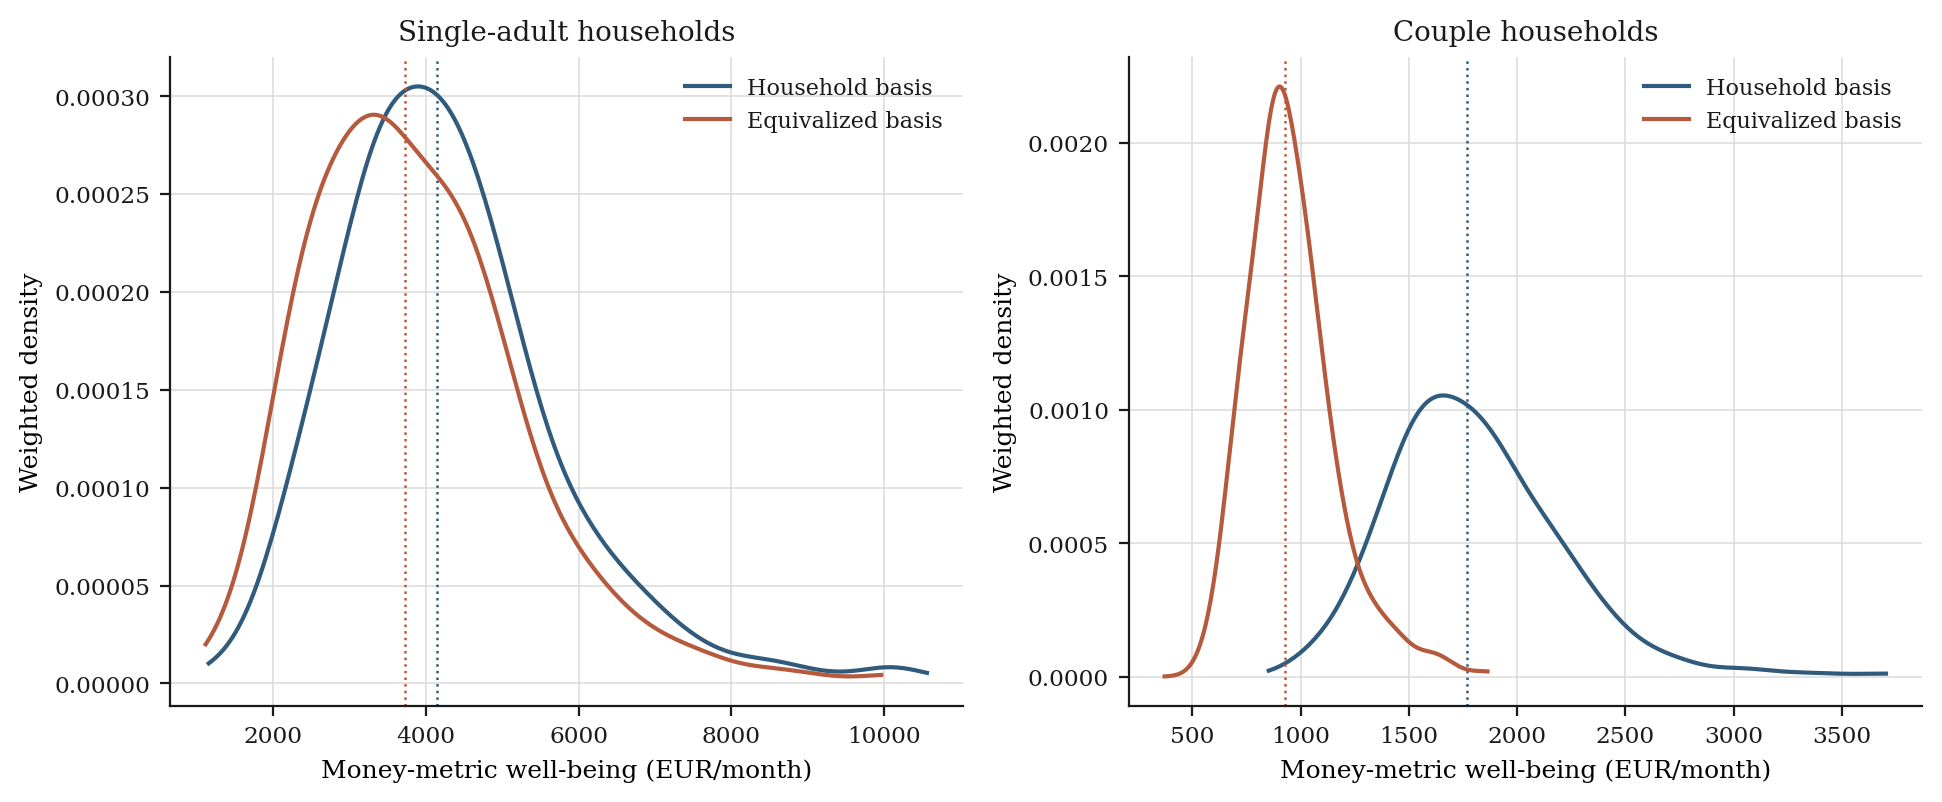
\includegraphics[width=0.95\linewidth,height=\textheight,keepaspectratio,alt={The distribution of money-metric well-being, by household type and basis, with weighted medians marked. Levels are not comparable across the two panels: each household type carries its own reference construction.}]{figures/v5/figV02_welfare_distributions.png}
\caption{The distribution of money-metric well-being, by household type and basis, with weighted medians marked. Levels are not comparable across the two panels: each household type carries its own reference construction.}
\end{figure}

\begin{figure}[H]
\centering
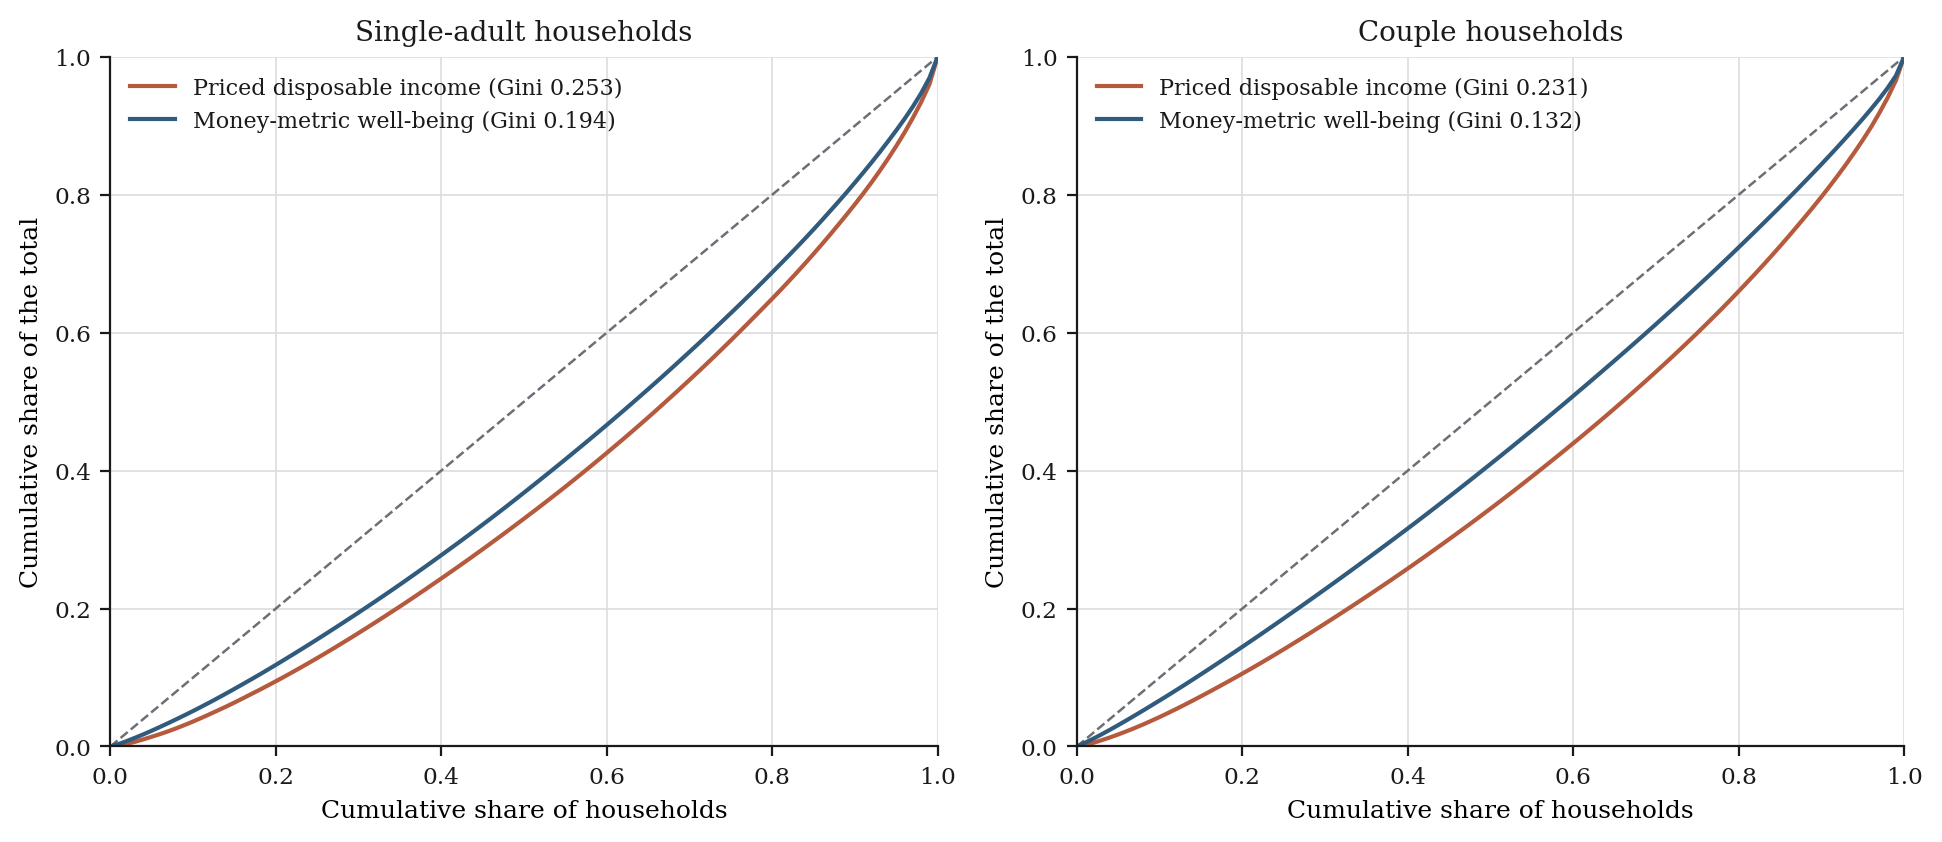
\includegraphics[width=0.95\linewidth,height=\textheight,keepaspectratio,alt={Lorenz curves of money-metric well-being and of the priced disposable income it replaces, over the same households and the same weights. The two curves answer different questions about the same households; their Gini values are not two estimates of one quantity.}]{figures/v5/figV01_welfare_lorenz.png}
\caption{Lorenz curves of money-metric well-being and of the priced disposable income it replaces, over the same households and the same weights. The two curves answer different questions about the same households; their Gini values are not two estimates of one quantity.}
\end{figure}

The money metric is less unequal than the priced disposable income it replaces, for both household types: the Gini falls from 0.253 to 0.194 for single adults and from 0.231 to 0.132 for couples. The two Ginis are not two estimates of one quantity. The income Gini describes an outcome; the welfare Gini describes an ex-ante monetary level built from each household's own preferences and own reachable jobs, and the difference between them is not a correction but a change of object.

Levels differ from income in opposite directions for the two types, and the levels are not comparable between them: each application carries its own reference construction, with a female-primary reference block for single adults and a medoid-spouse reference for couples, and the couples index adds two leisure terms. We use levels only within type and offer no mechanism for the between-type difference in levels.

